%package list
\documentclass{article}
\usepackage[top=3cm, bottom=3cm, outer=3cm, inner=3cm]{geometry}
\usepackage{multicol}
\usepackage{graphicx}
\usepackage{url}
%\usepackage{cite}
\usepackage{hyperref}
\usepackage{array}
%\usepackage{multicol}
\newcolumntype{x}[1]{>{\centering\arraybackslash\hspace{0pt}}p{#1}}
\usepackage{natbib}
\usepackage{pdfpages}
\usepackage{multirow}
\usepackage[normalem]{ulem}
\useunder{\uline}{\ul}{}
\usepackage{svg}
\usepackage{xcolor}
\usepackage{listings}
\lstdefinestyle{ascii-tree}{
    literate={├}{|}1 {─}{--}1 {└}{+}1 
  }
\lstset{basicstyle=\ttfamily,
  showstringspaces=false,
  commentstyle=\color{red},
  keywordstyle=\color{blue}
}
%\usepackage{booktabs}
\usepackage{caption}
\usepackage{subcaption}
\usepackage{float}
\usepackage{array}

\newcolumntype{M}[1]{>{\centering\arraybackslash}m{#1}}
\newcolumntype{N}{@{}m{0pt}@{}}


%%%%%%%%%%%%%%%%%%%%%%%%%%%%%%%%%%%%%%%%%%%%%%%%%%%%%%%%%%%%%%%%%%%%%%%%%%%%
%%%%%%%%%%%%%%%%%%%%%%%%%%%%%%%%%%%%%%%%%%%%%%%%%%%%%%%%%%%%%%%%%%%%%%%%%%%%
\newcommand{\itemEmail}{  \newline aanazcoh@unsa.edu.pe\newline  fvilcaqui@unsa.edu.pe \newline mhuamanivar@unsa.edu.pe \newline jturpoan@unsa.edu.pe}
\newcommand{\itemStudent}{Andre Renzo Añazco Huamanquispe\newline Frank's vilca Quispe\newline Melsy Melany Huamani Vargas \newline Jhamil Yeyder Turpo Añasco \newline}
\newcommand{\itemCourse}{Programación}
\newcommand{\itemCourseCode}{20231001}
\newcommand{\itemSemester}{III}
\newcommand{\itemUniversity}{Universidad Nacional de San Agustín de Arequipa}
\newcommand{\itemFaculty}{Facultad de Ingeniería de Producción y Servicios}
\newcommand{\itemDepartment}{Departamento Académico de Ingeniería de Sistemas e Informática}
\newcommand{\itemSchool}{Escuela Profesional de Ingeniería de Sistemas}
\newcommand{\itemAcademic}{2023 - A}
\newcommand{\itemInput}{Del 19 Junio 2023}
\newcommand{\itemOutput}{Al 19 Julio 2023}
\newcommand{\itemPracticeNumber}{05}
\newcommand{\itemTheme}{Django}
%%%%%%%%%%%%%%%%%%%%%%%%%%%%%%%%%%%%%%%%%%%%%%%%%%%%%%%%%%%%%%%%%%%%%%%%%%%%
%%%%%%%%%%%%%%%%%%%%%%%%%%%%%%%%%%%%%%%%%%%%%%%%%%%%%%%%%%%%%%%%%%%%%%%%%%%%

\usepackage[english,spanish]{babel}
\usepackage[utf8]{inputenc}
\AtBeginDocument{\selectlanguage{spanish}}
\renewcommand{\figurename}{Figura}
\renewcommand{\refname}{Referencias}
\renewcommand{\tablename}{Tabla} %esto no funciona cuando se usa babel
\AtBeginDocument{%
	\renewcommand\tablename{Tabla}
}

\usepackage{fancyhdr}
\pagestyle{fancy}
\fancyhf{}
\setlength{\headheight}{30pt}
\renewcommand{\headrulewidth}{1pt}
\renewcommand{\footrulewidth}{1pt}
\fancyhead[L]{\raisebox{-0.2\height}{
\includegraphics[width=3cm]{img/logo_episunsa.png}}}
\fancyhead[C]{\fontsize{7}{7}\selectfont	\itemUniversity \\ \itemFaculty \\ \itemDepartment \\ \itemSchool \\ \textbf{\itemCourse}}
\fancyhead[R]{\raisebox{-0.2\height}{
\includegraphics[width=1.2cm]{img/logo_abet}}}
\fancyfoot[L]{Estudiante Juan Perez Perez}
\fancyfoot[C]{\itemCourse}
\fancyfoot[R]{Página \thepage}

% para el codigo fuente
\usepackage{listings}
\usepackage{color, colortbl}
\definecolor{dkgreen}{rgb}{0,0.6,0}
\definecolor{gray}{rgb}{0.5,0.5,0.5}
\definecolor{mauve}{rgb}{0.58,0,0.82}
\definecolor{codebackground}{rgb}{0.95, 0.95, 0.92}
\definecolor{tablebackground}{rgb}{0.8, 0, 0}

\lstset{frame=tb,
	language=bash,
	aboveskip=3mm,
	belowskip=3mm,
	showstringspaces=false,
	columns=flexible,
	basicstyle={\small\ttfamily},
	numbers=none,
	numberstyle=\tiny\color{gray},
	keywordstyle=\color{blue},
	commentstyle=\color{dkgreen},
	stringstyle=\color{mauve},
	breaklines=true,
	breakatwhitespace=true,
	tabsize=3,
	backgroundcolor= \color{codebackground},
}

\begin{document}
	
	\vspace*{10px}
	
	\begin{center}	
		\fontsize{17}{17} \textbf{ Informe de Laboratorio \itemPracticeNumber}
	\end{center}
	\centerline{\textbf{\Large Tema: \itemTheme}}
	%\vspace*{0.5cm}	

	\begin{flushright}
		\begin{tabular}{|M{2.5cm}|N|}
			\hline 
			\rowcolor{tablebackground}
			\color{white} \textbf{Nota}  \\
			\hline 
			     \\[30pt]
			\hline 			
		\end{tabular}
	\end{flushright}	

	\begin{table}[H]
		\begin{tabular}{|x{4.7cm}|x{4.8cm}|x{4.8cm}|}
			\hline 
			\rowcolor{tablebackground}
			\color{white} \textbf{Estudiante} & \color{white}\textbf{Escuela}  & \color{white}\textbf{Asignatura}   \\
			\hline 
			{\itemStudent \par \itemEmail} & \itemSchool & {\itemCourse \par Semestre: \itemSemester \par Código: \itemCourseCode}     \\
			\hline 			
		\end{tabular}
	\end{table}		
	
	\begin{table}[H]
		\begin{tabular}{|x{4.7cm}|x{4.8cm}|x{4.8cm}|}
			\hline 
			\rowcolor{tablebackground}
			\color{white}\textbf{Laboratorio} & \color{white}\textbf{Tema}  & \color{white}\textbf{Duración}   \\
			\hline 
			\itemPracticeNumber & \itemTheme & 04 horas   \\
			\hline 
		\end{tabular}
	\end{table}
	
	\begin{table}[H]
		\begin{tabular}{|x{4.7cm}|x{4.8cm}|x{4.8cm}|}
			\hline 
			\rowcolor{tablebackground}
			\color{white}\textbf{Semestre académico} & \color{white}\textbf{Fecha de inicio}  & \color{white}\textbf{Fecha de entrega}   \\
			\hline 
			\itemAcademic & \itemInput &  \itemOutput  \\
			\hline 
		\end{tabular}
	\end{table}
	
\section*{\begin{center}
	Primer Avance de Nuestro Proyecto con Ayuda de Django
\end{center}}

\section{RESUMEN}
\begin{itemize}
\item 		El consorcio de construcción llamado San Antonio es una empresa que se dedica a proyectos de construcción en la ciudad del mismo nombre. Sin embargo, parece que hay un aspecto importante que aún no han implementado en su operación: un sistema para registrar charlas y entregar equipos de protección personal (EPPs).
            El registro de charlas es una práctica común en la industria de la construcción y tiene como objetivo principal garantizar la seguridad de los trabajadores. Durante estas charlas, se proporciona información sobre los riesgos laborales específicos del proyecto y se enseñan las medidas de seguridad necesarias para prevenir accidentes. Al no contar con un sistema para registrar estas charlas, San Antonio puede estar perdiendo la oportunidad de asegurarse de que todos sus trabajadores estén debidamente informados y capacitados para realizar sus tareas de manera segura.
\end{itemize}
\section{INTRODUCCIÓN}
\begin{itemize}
\item El consorcio de construcción San Antonio ha identificado una importante brecha en su operación: la ausencia de un sistema para registrar charlas de seguridad y entregar equipos de protección personal (EPPs) a sus trabajadores. Como estudiantes de Ingenieria de Sistemas, hemos decidido ayudar para crear un sistema personalizado que aborde estas necesidades utilizando Django, un framework web altamente confiable y escalable.

Nuestro objetivo es proporcionar a San Antonio una solución efectiva y eficiente que les permita programar y registrar charlas de seguridad de manera adecuada. Además, el sistema facilitará la entrega y el control de los EPPs necesarios para cada trabajador. Al aprovechar las capacidades de Django, garantizaremos la confiabilidad y la escalabilidad del sistema, lo que permitirá a San Antonio gestionar estas importantes tareas de manera eficiente.

Al implementar este nuevo sistema, San Antonio mejorará significativamente sus prácticas de seguridad laboral y asegurará que todos los trabajadores estén debidamente informados y equipados para realizar sus tareas de manera segura. Nuestra experiencia en el desarrollo de soluciones personalizadas utilizando Django nos permitirá cumplir con los requisitos específicos de San Antonio y brindarles una herramienta poderosa para fortalecer su enfoque en la seguridad en el lugar de trabajo.
\end{itemize}

\section{OBJETIVOS}
\begin{itemize}
\item
Registro de charlas de seguridad: Implementar un sistema que permita programar, registrar y gestionar las charlas de seguridad realizadas en el consorcio San Antonio. Esto incluirá la capacidad de programar fechas, registrar asistentes y mantener un registro de las charlas realizadas.

\item
Gestión de EPPs: Desarrollar un módulo que permita llevar un control efectivo de los equipos de protección  personal (EPPs) entregados a los trabajadores. Esto implicará la capacidad de solicitar, rastrear y registrar la entrega de los EPPs a cada trabajador, garantizando su disponibilidad y seguimiento adecuado.
\end{itemize}
\section{MÉTODO}
\begin{itemize}
\item Python: Python es un lenguaje de programación de alto nivel, interpretado y de propósito general. Con una sintaxis clara y legible, Python se destaca por su facilidad de uso y su enfoque en la legibilidad del código. Es un lenguaje versátil que permite desarrollar una amplia gama de aplicaciones, desde aplicaciones web y científicas hasta automatización de tareas y análisis de datos. Python cuenta con una gran cantidad de bibliotecas y módulos disponibles, lo que facilita el desarrollo rápido y eficiente de aplicaciones. Además, su comunidad activa y su documentación extensa hacen de Python una opción popular entre los programadores de todo el mundo.
\item Visual Studio: Es un entorno de desarrollo integrado (IDE) creado por Microsoft. Ofrece una amplia gama de herramientas y características para facilitar la programación en diversos lenguajes, como C#, C++, Python y más. Visual Studio proporciona un editor de código robusto con resaltado de sintaxis, depuración avanzada, autocompletado y control de versiones integrado. También ofrece una amplia variedad de plantillas y frameworks para acelerar el desarrollo de aplicaciones. Con su interfaz intuitiva y extensibilidad, Visual Studio se ha convertido en una opción popular para los desarrolladores que buscan un entorno completo y eficiente para crear aplicaciones de software de alta calidad.

\item Django es un framework web de alto nivel basado en Python que permite el desarrollo rápido y eficiente de aplicaciones web. Proporciona una arquitectura sólida y un conjunto de herramientas integradas que simplifican la creación de aplicaciones web seguras y escalables. Django ofrece características como el enrutamiento de URLs, un ORM (Mapeo Objeto-Relacional) para interactuar con la base de datos, un sistema de plantillas y una administración de contenido incorporada. Además, su enfoque en la legibilidad del código y la reutilización de componentes facilita la creación de aplicaciones mantenibles y extensibles. Django es ampliamente utilizado y respaldado por una comunidad activa, lo que brinda soporte y recursos adicionales para los desarrolladores.

\end{itemize}	
\begin{lstlisting}[language=bash,caption={Creando directorio de trabajo}][H]
		$ mkdir -p $HOME/rescobedoq/
	\end{lstlisting}
	
	\begin{figure}[H]
		%\centering
		%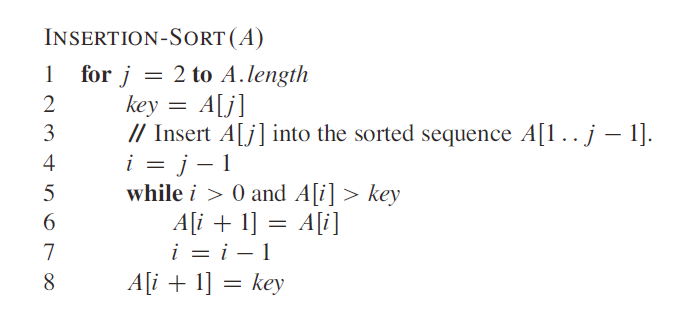
\includegraphics[width=0.8\textwidth,keepaspectratio]{img/pseudocodigo_insercion.png}
		%\includesvg{img/automata.svg}
		%\label{img:mot2}
		%\caption{Product backlog.}
	\end{figure}
	
	\lstinputlisting[language=Java, caption={Insertion.java},numbers=left,]{}
	
\section{RESULTADOS}
	\begin{itemize}	
		\item Texto...
	\end{itemize}
	

\section*{\textcolor{red}{REFERENCIAS}}
\begin{itemize}			
	\item \url{https://www.w3schools.com/java/default.asp}
	\item \url{https://www.geeksforgeeks.org/insertion-sort/}
\end{itemize}	
	
%\clearpage
%\bibliographystyle{apalike}
%\bibliographystyle{IEEEtranN}
%\bibliography{bibliography}
			
\end{document}
